% This file was converted to LaTeX by Writer2LaTeX ver. 1.0.2
% see http://writer2latex.sourceforge.net for more info
\documentclass{article}
\usepackage[utf8]{inputenc}
\usepackage[T1]{fontenc}
\usepackage[english]{babel}
\usepackage{amsmath}
\usepackage{amssymb,amsfonts,textcomp}
\usepackage{array}
\usepackage{hhline}
\usepackage[pdftex]{graphicx}
\author{till }
\date{2013-04-30}
\begin{document}
OOR / Ontohub API


\bigskip


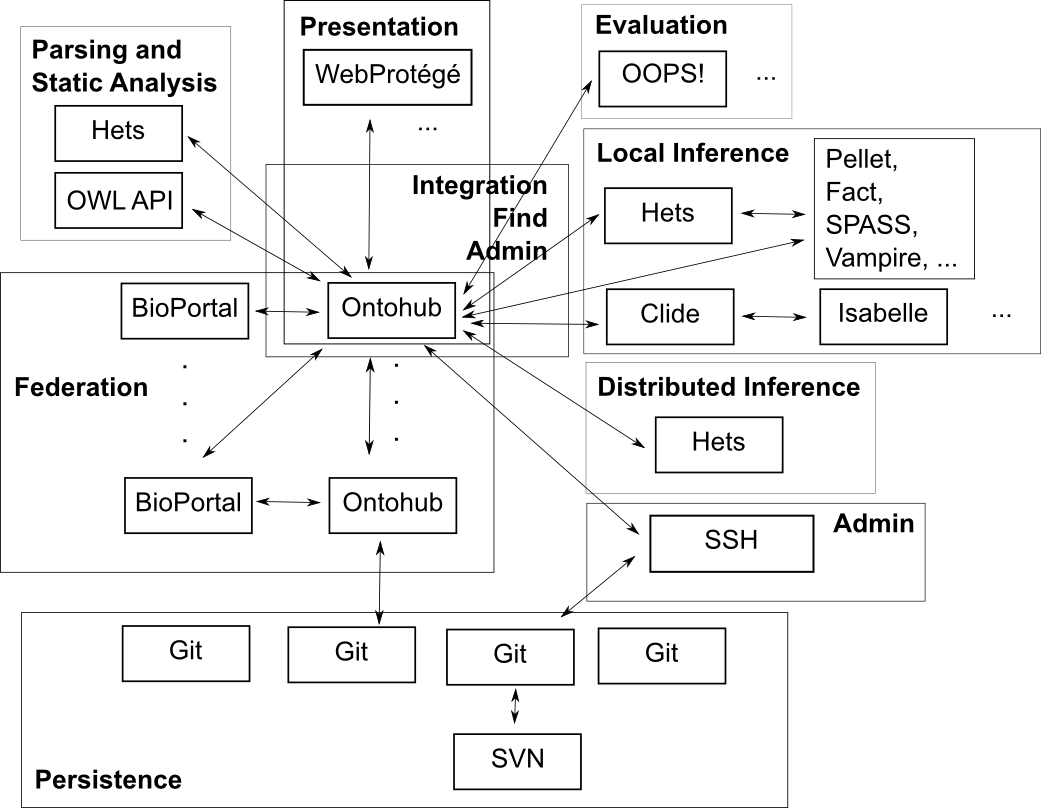
\includegraphics[width=15.822cm,height=12.277cm]{OOROntohubAPI-img1.png}


Federation and general

General remark: Any ontology and any link can be optionally accompanied
by a version id.

Ontology ids are instance specific



\bigskip

Ontology Services




\bigskip

Not formalized in OORService

\ \ \ index OntologyVersion\ \ \ \ (ontology[id,vid])\ \ $\Rightarrow$
(ontology)

&find Ontology SymbolsAndSentences

&(ontology[id])&$\Rightarrow$ (list(symbol), list(sentence))

&find OntologyVersion SymbolsAndSentences

&(ontology[id,vid])&$\Rightarrow$ (list(symbol), list(sentence))

&get Ontology Prefix&(ontology[id])&$\Rightarrow$
(prefix)

&list Categories&()&$\Rightarrow$ (list
(category[id,name])

&find Category Ontologies&(category[id])&$\Rightarrow$
(list (ontology[id,name])

&list Groups&()&$\Rightarrow$ (list
(group[id,name])

&find Language Ontologies&(language[id])&$\Rightarrow$
(list (ontology[id,name])


\bigskip

&upload OntologyVersion&(ontology[id],file)&$\Rightarrow$
(vid)

download OntologyVersion&(ontology[id,vid])&$\Rightarrow$
(file)


\bigskip


\bigskip


\bigskip

Formalized in OORService

\# not to be implemented in our system


\bigskip

Ontology

&find Ontology&(name{}-fragment) &$\Rightarrow$
(list (ontology[id,name]))

&create Ontology&(ontology) &$\Rightarrow$
(ontology[id])

&index Ontology&(ontology[id]) &$\Rightarrow$
(ontology)

&update Ontology&(ontology) &$\Rightarrow$ ()

&delete Ontology&(ontology[id]) &$\Rightarrow$ ()


\bigskip

&get OntologyVersion
Metrics&(ontology[id,vid])&$\Rightarrow$ (metrics)

&update OntologyVersion
Metrics&(ontology[id,vid],metrics)&$\Rightarrow$ ()

\ extract OntologyVersion
Metrics&(ontology[id,vid])&$\Rightarrow$ (metrics)


\bigskip

&get OntologyVersion
File&(ontology[id,vid,sid])&$\Rightarrow$ (file)

&find Latest OntologyVersions

&find Latest ActiveOntologyVersions


\bigskip

Note/Comment

&get AllNotes ForOnto&(ontology[id])&$\Rightarrow$
(list (note))

&get AllNotes ForOnto ByAuthor&(o[id],
author[id])&$\Rightarrow$ (list (note))

&get AllNotes ForConcept&(o[id],
concept[id])&$\Rightarrow$ (list (note))

&get AllNotes ForIndividual&(o[id],
indiv.[id])&$\Rightarrow$ (list (note))

&get AllNotes ForNote&(o[id],
note[id])&$\Rightarrow$ (list (note))

&create Note

&update Note

&archive Note

&delete Note

unarchive Note

&get Note Bean

&get RootNote

&archive Thread

unarchive Thread


\bigskip

Project

&create Project

\ retrieve Project

&update Project

&delete Project


\bigskip

Review

&create Review

\ retrieve Review

&update Review

&delete Review

&get Reviews ForOnto


\bigskip

Rating

&create Rating

&update Rating

&delete Rating

&get AllRatingTypes

\ retrieve RatingType


\bigskip

Finding Commands

&find OntologyOrView&$\Rightarrow$ find Ontology

&find LatestActiveOntologyVersions&$\Rightarrow$ find
LatestActiveOntologyVersions

&find LatestOntologyVersions&$\Rightarrow$ find
LatestOntologyVersions


\bigskip

cleanupOntologyCategory

getOntologyFile


Search

There is only one method (search), having the following parameters:

\begin{itemize}
\item search string (with Boolean operators and wildcards, e.g.
{\textquotedbl}foo bar -baz{\textquotedbl} will expand to
{\textquotedbl}foo* AND bar* AND NOT baz*{\textquotedbl})
\item
ontologyids={\textless}ontologyid{\textgreater},{\textless}ontologyid{\textgreater}…
- limits the search to specific ontologies (default: all ontologies)
\item searchontologynames=[1/0] – search in the ontology names (default:
1)
\item searchsymbolnames=[1/0] – search in the symbol names (default: 1)
\item isexactmatch=[1/0] – match the entire ontology resp. symbol name
(default: 0)
\item pagesize={\textless}pagesize{\textgreater} - the number of results
to display in a single request (default: all)
\item pagenum={\textless}pagenum{\textgreater} - the page number to
display (pages are calculated using {\textless}total
results{\textgreater}/{\textless}pagesize{\textgreater}) (default: 1)
\item maxnumhits={\textless}maxnumhits{\textgreater} - the maximum
number of top matching results to return (default: 1000)
\item symbolkinds={\textless}kind,kind,..{\textgreater} - limits the
results returned to these kinds, multitple kinds can be included in the
parameter.
\item includedefinitions=\{true\} - if a search result is a hit for a
symbol, adding this parameter will include the definition in the search
result xml.
\end{itemize}

\bigskip

Persistence

\begin{itemize}
\item Synchronize two repositories (also non-git ones, like triple
stores)
\end{itemize}
Difference

createDiff

createDiffForLatestActiveOntologyVersionPair

createDiffForAllActiveVersionsOfOntology

getAllDiffsForOntology

getDiffFileForOntologyVersions


Distributed Inference

Open question: should we use Hets development graph sessions, or only
send around updates to ontologies and links?

Here is the session based API:

\begin{itemize}
\item POST /libraries/{\textless}coded-iri{\textgreater}/sessions -
create a new proof session for development graph
\item GET
/sessions/{\textless}id{\textgreater}?format={\textless}f{\textgreater}
- get proof state of session
\item GET /menus - Get development graph menu structure
\item GET
/nodes/{\textless}coded-iri{\textgreater}?library={\textless}coded-iri{\textgreater}\&session=id
- Get info for node
\item GET
/nodes/{\textless}coded-iri{\textgreater}/theory?library={\textless}coded-iri{\textgreater}\&session=id
- Get theory of node
\item GET
/edges/{\textless}coded-iri{\textgreater}?library={\textless}coded-iri{\textgreater}\&session=id
- Get info for edge
\item PUT
/libraries/{\textless}coded-iri{\textgreater}/proofs/{\textless}id{\textgreater}/{\textless}command{\textgreater}
- execute command for session
\item PUT
/sessions/{\textless}id{\textgreater}/{\textless}command{\textgreater}?node={\textless}iri{\textgreater}\&edge={\textless}iri{\textgreater}-
execute command for node in session
\item GET
/sessions/{\textless}id{\textgreater}/provers?node={\textless}iri{\textgreater}\&translation={\textless}iri{\textgreater}
- Get provers for node
\item GET
/sessions/{\textless}id{\textgreater}/translations?node={\textless}iri{\textgreater}
- Get logic translations for node
\item PUT
/sessions/{\textless}id{\textgreater}/prove?node={\textless}iri{\textgreater}?prover={\textless}name{\textgreater}\&translation={\textless}iri{\textgreater}
\&timeout={\textless}secs{\textgreater}\&include=true - Call prover
\end{itemize}
List of available Hets commands (which ones do we need here?)

dg-all auto
&Apply
automatic tactic - needed 

dg-all glob-decomp &Apply rule
global-decomposition - to start with, auto should suffice

dg-all global-subsume &Apply rule global-subsumption
- to start with, auto should suffice

dg-all loc-decomp &Apply rule
local-decomposition - to start with, auto should suffice

dg-all local-infer &Apply rule
local-inference - to start with, auto should suffice

dg-all comp &prove
composed edges - to start with, auto should suffice

dg-all comp-new &create composed
proven edges - to start with, auto should suffice

dg-all cons
&Apply rule
conservativity - to start with, auto should suffice

dg-all hide-thm &Apply rule
hide-theorem-shift - to start with, auto should suffice

dg-all thm-hide &Apply rule
theorem-hide-shift - to start with, auto should suffice

compute-colimit &compute colimit -
not needed, since this is called by static analysis of “combine”

compute-normal-form &Compute normal forms for nodes
with incoming hiding links \ {}- needed for proving in presence of
hiding

triangle-cons
&triangle-cons -
needed

freeness
&freeness
- not needed in DOL

flattening importing &Flatten all theories
and delete all importing links \ {}- needed for interfacing to standard
theorem provers

flattening disjoint-union &Create intersection nodes and
ensure only disjoint unions \ {}- needed for interfacing to some (but
not many) theorem provers

flattening renaming &Flatten out renaming
\ {}- needed for interfacing to some (but not many) theorem provers

flattening hiding &Delete all
hiding links \ {}- needed for interfacing to some (but not many)
theorem provers

flattening heterogeneity &Flatten out heterogeneity -
needed for interfacing to some (but not many) theorem provers

qualify-all-names &Qualify and
disambiguate all signature names

undo
&Undo
last change - not needed

redo
&Redo
last change - not needed

use
&{\textless}File{\textgreater}
&Read HetCASL file - not needed

dg basic
&{\textless}Nodes{\textgreater}
&Select node - needed

translate
&{\textless}Comorphism{\textgreater}
\ Choose translation - needed

prover
&{\textless}Prover{\textgreater}
&Choose prover - needed

set goals
&{\textless}Goal{\textgreater}
&Set goal - needed

prove
&Applies
selected prover to selected goals - needed

check-consistency &check
consistency - needed

drop-translations &Drops
any selected comorphism - needed

cons-checker
&{\textless}ConsChecker{\textgreater} Choose
consistency checker - needed

conservativity-check &{\textless}Edges{\textgreater}
&Choose conservativity checker - needed

set time-limit &{\textless}Number{\textgreater}
&Set the time-limit for the next proof - needed

set axioms
&{\textless}Axiom{\textgreater}
&Set the axioms used for the next proof - needed

set include-theorems true &Include proven
theorems - needed

set include-theorems false &Do not include
proven theorems - needed

nodes
&Show
Nodes - not needed

edges
&Show
Edges - not needed

show-undo-history &Show
Undo-History - not needed

show-redo-history &Show
Redo-History - not needed

show-proven-goals-current &Show Proven
Goals of selected node - needed

show-unproven-goals-current &Show Unproven Goals of
selected node - needed

show-all-axioms-current &Show All
Axioms of selected node - needed

show-all-goals-current &Show All
Goals of selected node - needed

show-computed-theory-current &Show Computed Theory of
selected node - needed

show-taxonomy-current &Show
Taxonomy of selected node - not needed

show-concept-current &Show
Concept of selected node - not needed

show-node-info-current &Show
Node-Info of selected node - needed

show-node-info &{\textless}Nodes{\textgreater}
&Show Node-Info - needed

show-computed-theory &{\textless}Nodes{\textgreater}
&Show Computed Theory - needed

show-all-goals &{\textless}Nodes{\textgreater}
&Show All Goals - needed

show-proven-goals &{\textless}Nodes{\textgreater}
&Show Proven Goals - needed

show-unproven-goals &{\textless}Nodes{\textgreater}
&Show Unproven Goals - needed

show-all-axioms &{\textless}Nodes{\textgreater}
&Show All Axioms - needed

show-taxonomy &{\textless}Nodes{\textgreater}
&Show Taxonomy - not needed

show-concept &{\textless}Nodes{\textgreater}
&Show Concept - not needed

show-edge-info &{\textless}Edges{\textgreater}
&Show Edge-Info - needed

expand
&Extend
current node - ???

addview
&Add a
view - ???

help
&Show
all available commands - see DG menus?

quit
&Quit
- not needed


\bigskip


\bigskip

Here is an API for sending around updates:

\begin{itemize}
\item prove link. Input: IRI of link. Output: list of new links and/or
proof goals for simple ontologies that will prove the link
\end{itemize}

\bigskip


\bigskip


\bigskip

Evaluation and other services

OOPS! and similar services

we propose the following abstraction from the OOPS! API:

input: ontology\footnote{\ OOPS! has more inputs, but we let the list of
pitfalls empty, and the output format be XML.}

output: list of response elements of the following form:

type (for OOPS: pitfall, warning, suggestion)

code (an integer)

name

description

list of involved symbols\footnote{\ OOPS! outputs structured XML
elements that may contain multiple n{}-ary relations between symbols
(e.g. oops:MightBeEquivalentProperty and
oops:MightBeEquivalentAttribute). We prefer to have only one such
relation per response element.}


\bigskip

Annotator Service


\bigskip

This service it specific to bio ontologies. How to generalise it to
other domains? It seems that some (more static) list of service types
and (more dynamically growing) list of actual services (conforming to
these service types) would be useful. This of course also includes
services like OOPS!


\bigskip

Ontology Recommender


\bigskip

Interesting challenge to generalise this to ontologies written in
arbitrary languages...


\bigskip

Resource Index Service


\bigskip

could be adapted for Ontohub, if {\textquotedbl}concept{\textquotedbl}
is replaced by {\textquotedbl}symbol{\textquotedbl}


\bigskip

Notes Service (Term Proposals and Comments)


\bigskip

Logic-specific services

OWL specific services involving the class hierarchy

These services could also be used for other languages if there is a
suitable projection to OWL.


\bigskip

Remaining stuff from OOR

&find AllOntologyOrViewVersionsByVirtualId\#

&find LatestAutoPulledOntologyVersions\#

&find LatestActiveOntologyOrViewVersion\#

&find LatestActiveOntologyViewVersions\#

&find LatestOntologyOrViewVersion\#

& find LatestOntologyViewVersions\#


\bigskip
\end{document}
